\subsection{Complessità di un Problema}
Dato un problema P \{INPUT $\rightarrow$ OUTPUT\}, la \textbf{complessità} di P è la 
complessità dell'algoritmo più efficiente che risolve P.

\paragraph{Limite superiore per complessità di P} Se A è un algoritmo per P con
complessità  $O \big( f(n) \big)$, allora P è $O \big( f(n) \big)$.

\paragraph{Limite inferiore per complessità di P}
Se ogni algoritmo che risolve P ha complessità $\Omega \big( f(n) \big)$, allora 
P ha complessità $\Omega \big( f(n) \big)$
\bigskip

$\implies$ se P è $O \big( f(n) \big)$ e $\Omega \big( f(n) \big) \Rightarrow$ P è $\Theta \big( f(n) \big)$ 

\subsubsection{Esempio: limite inferiore per ordinamento basato su scambi di elementi contigui}

\paragraph{Def (inversione)} Dato \texttt{A[1$\twodots$n]}, una \emph{inversione} è una coppia $(i,j)$
con $i,j \in [1,n]$ con $i < j$ e \texttt{A[i]} $>$ \texttt{A[j]}.\par \medskip
Operazione disponibile: \texttt{A[k]} $\leftrightarrow$ \texttt{A[k+1]} (scambio tra gli elementi in posizione
$k$ e $k+1$).
\begin{align*}
	\# inv(A) & = \text{numero di inversioni di } A \\
	& = \Big{\vert} \ \{ (i,j) : 1 \leq i \leq j \leq n, \ A[i] > A[j] \} \ \Big{\vert}
\end{align*}

\begin{enumerate}
	\item A è ordinato sse $\# inv(A) = 0$;
	\item A è ordinato in senso inverso sse 
	\begin{displaymath}
		\displaystyle\sum_{j=2}^{n}j-1 = \displaystyle\sum_{j=1}^{n-1}j = \frac{n(n-1)}{2}
	\end{displaymath}
	Ossia, $\# inv(A)$ è massimizzato.
\end{enumerate}

Vediamo cosa succede alle coppie $(i,j)$ e a $\# inv(A)$ nel caso avvenga uno scambio \texttt{A[k]}
$\leftrightarrow$ \texttt{A[k+1]}.

\begin{itemize}
	\item $i,j \neq k$ e $i,j \neq k+1 \implies (i,j)$ è inversione prima sse è inversione dopo;
	\item $i = k, \ j = k+1$
	\[ \implies
	\begin{cases}
		A[i] < A[j] & \quad +1 \text{ inversione} \\
		A[i] = A[j] & \quad \# inv(A) \text{ non cambia} \\
		A[i] > A[j] & \quad -1 \text{ inversione}
	\end{cases}
	\]
	\item $i = k$ oppure $i = k+1$, $j > k+1 \implies (k,j)$ è inversione prima sse $(k+1,j)$ è
	inversione dopo;
	\item $j = k$ oppure $j = k+1$, $i < k$, analogo al caso precedente.
\end{itemize}

Per concludere, possiamo dire che l'operazione \texttt{A[k]} $\leftrightarrow$ \texttt{A[k+1]}
riduce $\# inv(A)$ al massimo di 1.
\begin{displaymath}
	\implies \text{qualunque algoritmo di ordinamento basato su scambi è } \Omega \Big(\frac{n(n-1)}{2} \Big) = \Omega (n^2)
\end{displaymath}

\subsection{Soluzione di Ricorrenze}
Abbiamo visto per \texttt{Merge Sort} la complessità nel modo seguente:

\begin{codebox}
	\Procname{$\proc{Merge-Sort}(A,p,r)$}
	\li \If $p < r$
	\li     \Then
	$q \gets \floor{\frac{(p + r)}{2}}$ 
	\li         $\proc{Merge-Sort}(A,p,q)$
	\li         $\proc{Merge-Sort}(A,q+1,r)$
	\li         $\proc{Merge}(A,p,q,r)$
	\Comment complessità $an + b$
	\End
\end{codebox}

\[ T^{MS}(n) =
\begin{cases}
c_0       & \quad \text{se } n \leq 1 \\
T^{MS}(\floor{\frac{n}{2}})+T^{MS}(\ceil{\frac{n}{2}}) + an + b  & \quad \text{se } n>1
\end{cases}
\]

È stato tuttavia un approccio non molto preciso. Ci sono due metodi per risolvere precisamente 
i problemi di ricorrenza:
\begin{itemize}[noitemsep]
	\item \emph{Metodo di sostituzione} (\ref{ricorrenze:sostituzione});
	\item \emph{Master Theorem} (\ref{mastertheorem}).
\end{itemize}

\subsubsection{Metodo di Sostituzione} \label{ricorrenze:sostituzione}
Dato una ricorrenza, si può provare a ``indovinare'' la soluzione e dimostrare che è corretta, oppure si può sviluppare l'\emph{albero %
delle ricorrenze}:
\begin{itemize}
	\item \emph{radice}: chiamata di cui vogliamo la complessità;
	\item per ogni nodo:
	\begin{itemize}
		\item[$\rightarrow$] costo della parte non ricorsiva;
		\item[$\rightarrow$] un figlio per ogni chiamata.
	\end{itemize}
\end{itemize}

\paragraph{Esempio} 

\[ T(n) =
\begin{cases}
4       & \quad \text{se } n = 1 \\
2T(\dfrac{n}{2})+ 6n  & \quad \text{se } n>1
\end{cases}
\]

In generale, si può benissimo trascurare il caso base per poter ottenere espressioni meno verbose, in questo 
caso otterremmo:
\begin{displaymath}
	T(n) = 2T(\frac{n}{2})+ 6n
\end{displaymath}

Costruendo l'albero delle ricorrenze si intuisce già la soluzione:
\begin{center}
	\begin{tikzpicture}
	\tikzset{every tree node/.style={align=center,anchor=north}}
	\tikzset{level 1/.style={level distance=40pt}}
	\tikzset{level 2/.style={level distance=70pt}}
	\tikzset{level 3/.style={level distance=70pt}}
	\tikzset{level 4/.style={level distance=30pt}}
	\Tree
	[.$T(n)$\\$6n$
	[.$T(\dfrac{n}{2})$\\$6\dfrac{n}{2}$
	[.$T(\dfrac{n}{4})$\\$6\dfrac{n}{4}$
	[.{\dots} \edge[dashed]; 4 ]
	[.{\dots} \edge[dashed]; 4 ]
	]
	[.$T(\dfrac{n}{4})$\\$6\dfrac{n}{4}$
	[.{\dots} \edge[dashed]; 4 ]
	[.{\dots} \edge[dashed]; 4 ]
	]
	]
	[.$T(\dfrac{n}{2})$\\$6\dfrac{n}{2}$
	[.$T(\dfrac{n}{4})$\\$6\dfrac{n}{4}$
	[.{\dots} \edge[dashed]; 4 ]
	[.{\dots} \edge[dashed]; 4 ]
	]
	[.$T(\dfrac{n}{4})$\\$6\dfrac{n}{4}$
	[.{\dots} \edge[dashed]; 4 ]
	[.{\dots} \edge[dashed]; 4 ]
	]
	]
	]
	\end{tikzpicture}
\end{center}
Tutte le foglie insieme costano $4n$. Ogni altro livello dell'albero costa $6n$, ma siccome l'altezza è circa $\log_2 n$, in totale costano $6n \log_2 n$. \\ 

Per essere sicuri della soluzione, facciamo il procedimento per intero.
Proviamo a ``indovinare'' la soluzione. Assomiglia a \texttt{Merge Sort},
quindi ipotizziamo abbia una complessità con un andamento simile 
\begin{displaymath}
	T(n) = an \log n + bn + c
\end{displaymath}
Facciamo la prova induttiva.

\begin{align*}
	(n = 1) \quad T(1) & = 4 \\
	& = a \cdot 1 \cdot \log 1 + b \cdot 1 + c  && (\log 1 = 0)\\
	& = b + c && \text{ok se } b + c = 4 \\
	(n > 1) \quad T(n) & = 2T \big( \frac{n}{2} \big) + 6n \\
\end{align*}
\begin{align*}
	\text{Per ipotesi induttiva} \\
	T \big( \frac{n}{2} \big) & = a \frac{n}{2} \cdot \log \frac{n}{2} + b \frac{n}{2} + c \\
	\text{Calcolo ora } T(n) \\
	T(n) & = an \log_2 \frac{n}{2} + bn + 2c + 6n = \\
	& = an \log_2n - an \log_22 + bn + 6n + 2c =  && (\log_22 = 1)\\
	& = an \log_2n + n(b + 6 - a) + 2c = \\
	& = an \log_2n + bn + c \\
	& \qquad \Downarrow
\end{align*}
\begin{align*}
	b + 6 - a = b \Rightarrow \ & a = 6 \\
	2c = c \Rightarrow \ & c = 0 \\
	& b + c = 4 \Rightarrow b = 4 \\
	T(n) &= an \log n + bn + c \\
	&= 6n \log n + 4n
\end{align*}